\documentclass[conference]{IEEEtran}
\IEEEoverridecommandlockouts
\usepackage{lipsum}
\linespread{1.5}
% The preceding line is only needed to identify funding in the first footnote. If that is unneeded, please comment it out.
\usepackage{cite}
\usepackage{amsmath,amssymb,amsfonts}
\usepackage{algorithmic}
\usepackage{graphicx}
\usepackage{textcomp}
\usepackage{xcolor}
\def\BibTeX{{\rm B\kern-.05em{\sc i\kern-.025em b}\kern-.08em
    T\kern-.1667em\lower.7ex\hbox{E}\kern-.125emX}}
    
    
\begin{document}

\title{ Plant-leaf disease recognition using Image Processing \\
{\footnotesize \textsuperscriptLogical Procedure and application techniques }
}

\author{
  \IEEEauthorblockN{1\textsuperscript{st} Anzum Kazi Tamrin}
\IEEEauthorblockA{\textit{Computer Science And Engineering} \\
\textit{American Intl. University Bangladesh}\\
Dhaka, Bangladesh \\
rahivjobs@gmail.com}
\and
  \IEEEauthorblockN{2\textsuperscript{nd} Samiya Nasir}
\IEEEauthorblockA{\textit{Computer Science And Engineering} \\
\textit{American Intl. University Bangladesh}\\
Dhaka, Bangladesh \\
samiyanasir1998@gmail.com }
\and
 \IEEEauthorblockN{3\textsuperscript{rd} Abedin Md Jobayer}
\IEEEauthorblockA{\textit{Computer Science And Engineering} \\
\textit{American Intl. University Bangladesh}\\
Dhaka, Bangladesh \\
jobayerabedin44@gmail.com}
\and


}






\maketitle

\begin{abstract}
Image processing is a method to perform operations in image or bitmap to extract meaningful and useful information from it. It can be applied on living things to analyze and inspect and gather data to perform scientific experiments. Identifying plants leaf disease in scale has been a very tedious job and very important in agricultural field and productivity on which our economy highly relies on.
\end{abstract}

%\begin{IEEEkeywords}
%component, formatting, style, styling, insert
%\end{IEEEkeywords}

\section{Introduction}
\large
 The techniques of image recognition are widely used on agricultural field and vastly important on the cultivation and crop protection field. Detecting plant infections or disease using not bare eyes but image processing is much beneficial as it saves a lot of time and human resource to monitor each and every plant thoroughly. Detecting the symptoms of the plant and the infection possibility detection is much more important to do infection prevention and to take security measurements before it appears on mass production.
\\
To detect and classify plant diseases there could be several ways and computational algorithms to help. Generally, we can observe the whole object thus the state and symptoms, so we will take plant leaves to analyze and identification of the affected plants.   



\section{Objective}
\large Recognizing plant leaves and detect diseases or infection is a challenging task to perform because generally they’re appeared on the plant stem or leaf area. Identifying the plant leaves using image processing is challenging and tough because there is so many problem domains and case studies to deal with. The first goal would be detecting a leaf first then differentiating a healthy leaf as and affected spotted leaves and then analyze the affected area by measuring the boundaries and match or decide possible results by valid disease symptoms and relevant data-sets.

Size, shape and color through times should be a concern to analyze regularities and irregularities of the plant leaves for better assumption and inspection.

The main objectives for this research would be:

\begin{itemize}
    \item	Recognizing disease using image processing.
    \item Making assumptions by analyzing the data sets.
    \item Experiment and observations.
    \item Making judgement following the observation and experimental data.
\end{itemize}



\section{Proposed method }
\large 
Quantitative research method could be a better fit for this research.  Based on numerical, statistical analysis and mining that information for better insights will help us to discover relativity and pattern recognition which will further help to generalize thoughts and take proper actions and approaches. This method technique harvests insights from surveys and queries with experimental approaches which can be used for observing and mining for research activities.

Size, shape and color through times should be a concern to analyze regularities and irregularities of the plant leaves for better assumption and inspection.

The main objectives for this research would be:

\begin{figure}
\centering
\caption{Workflow}
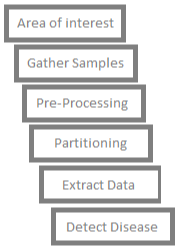
\includegraphics[scale=0.65]{workflow2.png}
\end{figure}

\vfill\null

\subsection{Area of Interest}
First of all, we have to figure out our area of interest, our area of concern, how to do and what would be our concern, that is already likely to be known as we are selecting leaf of a plant to analyze and proceed our research work.



\subsection{Gather Samples}
We have to gather samples, insights from various published documents and research works to not only extend but gather a better understanding from the previous work. So we have to collect plant leaves, affected leaves and not affected leaves and the transition leaves which will show us how likely the infection or disease occur over time.


\subsection{Pre-Processing}
Now we have to pre-process our data because as we are choosing the image processing approach, we have to work with noise reduction from image, color correction, image resize and error detection and filtering to a standard or normalized version which will likely to be standard to match our workflow or research progress.



\subsection{Partition}
After gathering samples and processing image, now we have to partition and classify our data set to maintain an order and distinction to better understandings.

\subsection{Extract Data}
We have to extract our valuable information throughout the findings to use in our experiment or research work.


\subsection{Detect Disease}
Now we have to detect plant leaf infections from the partitioned and extracted data sets using various image classifier and clustering algorithms. K-Means clustering algorithm can be used to analyze and distinct our findings to K number of groups. SVM (Support Vector Machine) could also be used which is based on statistical data sets which will help us to analyze certainty and uncertainty in our proposed scenario findings.

\subsection{Current Progress }
The work is currently one month and 3 days running under supervision of DR. M. M. MAHBUBUL SYEED. We now have our work proposed and explored our way to work and decided some best approaches for the research work. We have selected some classifier and clustering algorithms to analyze our image and datasets and selected some toolchains and programming algorithm and relevant libraries to proceed our work.


\begin{thebibliography}{00}
\bibitem{b1} Eduardo A.B. da Silva, and Gelson V. Mendonça, The Electrical Engineering Handbook April 2005. 
\bibitem{b2} K. Renugambal ,B. Senthilraja, 3rd Issue., vol. 4, March-2015
\bibitem{b3} Sujatha R*, Y Sravan Kumar and Garine Uma Akhil, 1st Issue., vol. 10, March-2017
\end{thebibliography}
\vspace{12pt}
\color{red}
\end{document}
